\section{Results and analysis}\label{sec:results}

\subsection{Real-world applications}\label{sec:res-apps}
Figure~\ref{fig:cases} and Table~\ref{tab:cases} show the three applications. In the two largest NASA defect sets, mc1 and pc2, about \NCsMcOnePi{} and \NCsPcTwoPi{} of test modules have an exact copy in the training data. The usual check looks fine: the random forest's 90\% sets covered \NCsMcOneReported{}\% and \NCsPcTwoReported{}\% of all test modules. New modules were covered only \NCsMcOneNew{}\% and \NCsPcTwoNew{}\% of the time. The check flags both data sets before training, with predicted gaps of \NCsMcOnePred{} and \NCsPcTwoPred{}\,pp. The observed gaps are smaller than this worst case, as expected for a model that does not memorize perfectly, but of the same order. Separate calibration brought new-module coverage to \NCsMcOneFixed{}\% and \NCsPcTwoFixed{}\%. In the intrusion data, \NCsKddPi{} of test connections have a training copy. New connections were covered \NCsKddNew{}\% of the time, and \NCsKddFixed{}\% with the fix. In the phishing data the figures were \NCsPhishNew{}\% and \NCsPhishFixed{}\%. Coverage must be read together with set size: LightGBM on the intrusion data reached high coverage only with sets of \NCsKddLgbmSize{} labels on average for new connections (Table~\ref{tab:cases}), which are of little use. The check flagged \NCsNFlagW{} of the \NCsNFlagTotal{} application data sets. Among the flagged sets, new-case coverage ranged from \NCsFlagNewRange{}\% without the fix and from \NCsFlagFixedRange{}\% with it.

The check is a warning, not a certainty, and it can miss. It flagged kc3 (predicted gap \NCsKcThreePred{}\,pp), but kc3's new modules were covered at \NCsKcThreeNew{}\% even without the fix. The check did not flag kc2 on its predicted gap (\NCsKcTwoPred{}\,pp), yet new modules there were covered at \NCsKcTwoNew{}\%. Its exposure (\NCsKcTwoPi{} of test rows seen) does trigger the combined rule. In the five other small defect sets, new-case coverage stayed within about 2\,pp of the target (\NCsSafeRange{}\%).

\begin{figure}[t]
\centering
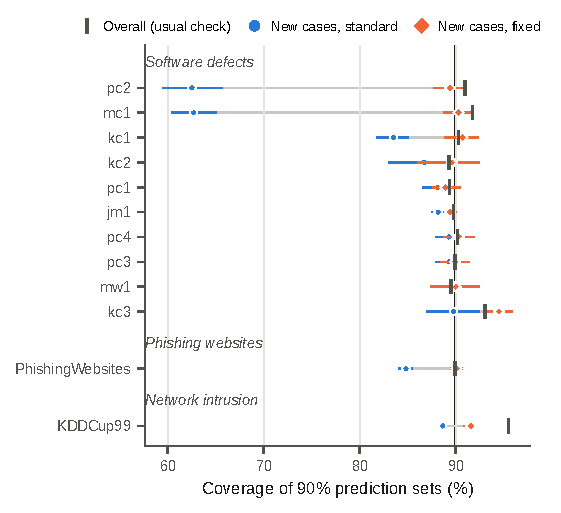
\includegraphics[width=0.62\textwidth]{figures/fig_cases.pdf}
\caption{In the three applications, the usual check reports about 90\% coverage while new cases are covered much less often, and separate calibration restores the target. Random forest, 90\% target, 10 random splits; error bars are 95\% bootstrap intervals of the mean over splits}\label{fig:cases}
\end{figure}

\begin{table}[t]
\caption{Applications at a 90\% target (random forest, RF, and LightGBM, LGBM; means over 10 random splits). Seen: share of test rows with an exact training copy. $g^*$: predicted gap from the check (no model). Overall: coverage reported by the usual check. New, std / New, fix: coverage of new cases without and with separate calibration. Size: mean set size for new cases, standard and fixed}\label{tab:cases}
\centering\scriptsize
\setlength{\tabcolsep}{2.5pt}
\begin{tabular}{@{}lcrrrrrr@{}}
\toprule
Data & Model & Seen (\%) & $g^*$ (pp) & Overall & New, std & New, fix & Size std\,/\,fix\\
\midrule
\tabinput{tables/tab_cases.tex}
\botrule
\end{tabular}
\end{table}

\subsection{Statistical analysis by hypothesis}\label{sec:res-hyp}

\paragraph{H1: the typical benchmark is not affected.} Repeated rows are common: \NNAnyDup{} of the \NNTotal{} benchmark data sets contain at least one, and in \NNDupGeThreeZero{} at least 30\% of rows belong to a group of identical rows. Exposure (Eq.~\ref{eq:exposure}) predicted the observed share of seen test rows almost exactly (mean absolute error \NExpMae{}). The planned test of a general shortfall was negative. The median new-case gap was between \NHOneGapMedianMin{} and \NHOneGapMedianMax{}\,pp across learner--score families, and no family was significant after Holm correction (smallest adjusted $p$ = \NHOneMinPHolm{}). Shortfalls were concentrated where many test rows are seen. Where at least 30\% are seen, \NXHiShareTwo{}\% of data set--learner pairs fell more than 2\,pp short and \NXHiShareFive{}\% more than 5\,pp. The worst gaps were \NHOneWorstGapCls{}\,pp (classification) and \NHOneWorstGapReg{}\,pp (regression).

\paragraph{H2: copies cause the shortfall.} Appending exact copies to the \NNdN{} duplicate-free data sets raised exposure as Eq.~(\ref{eq:exposure}) predicts, and the gap grew with it (Fig.~\ref{fig:inject}). For random forests in classification, the median gap went from \NInjClassificationRfZeroGap{}\,pp without copies to \NInjClassificationRfZeropFiveGap{}\,pp with half of the rows copied and \NInjClassificationRfOneGap{}\,pp with all rows copied. The regression figure with all rows copied was \NInjRegressionRfOneGap{}\,pp. LightGBM behaved similarly. Regularized linear models, which do not memorize rows, were barely affected (\NInjClassificationLogregOneGap{}\,pp). Separate calibration stayed at the target at every rate.

\begin{figure}[t]
\centering
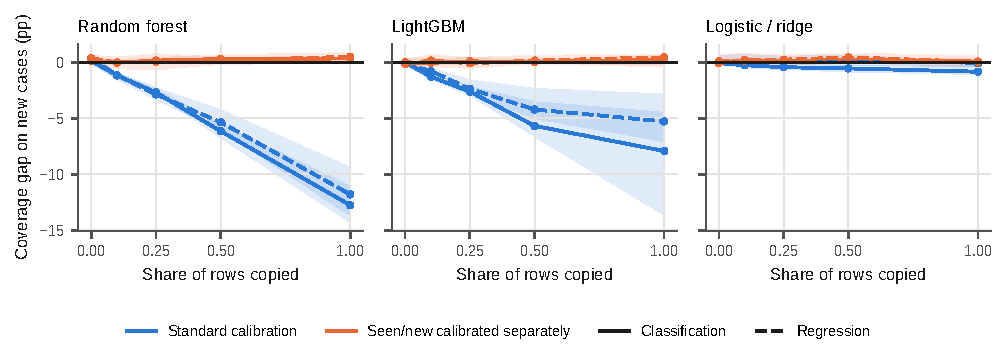
\includegraphics[width=\textwidth]{figures/fig_inject.pdf}
\caption{Copying rows on purpose creates the shortfall for flexible learners, in proportion to the share copied, while separate calibration stays on target. Median new-case gap over the \NNdN{} duplicate-free benchmark data sets; bands are 95\% bootstrap intervals of the median}\label{fig:inject}
\end{figure}

\paragraph{H3 and H4: the fix keeps its promise at little cost.} On the benchmarks with repeats, the median new-case gap of separate calibration ranged from \NHTwoMcpMedianRange{}\,pp, and the confidence interval of the median stayed above $-1$\,pp in \NHTwoNoninfAll{} learner--score combinations. Figure~\ref{fig:validity}a shows target against achieved coverage at three target levels. The overall coverage of standard calibration matches the target and its new-case coverage falls below it, while separate calibration matches the target for new cases. On the \NScpN{} fresh data sets (Fig.~\ref{fig:validity}b), the worst data set's gap with the fix was \NPrThreeRfMCPWorst{} (wave~1) and \NWTwoFixRfWorst{}\,pp (wave~2) for random forests. For LightGBM it was \NPrThreeLgbmMCPWorst{} and \NWTwoFixLgbmWorst{}\,pp, and for linear models \NPrThreeLogregMCPWorst{} and \NWTwoFixLogregWorst{}\,pp. Without the fix, the worst gaps were \NPrThreeRfSCPWorst{} and \NWTwoSCPRfWorst{}\,pp. The cost was small. On the benchmarks, sets for new cases grew by a median factor of \NHThreeNovelRatioRange{}, and on the wave-1 data by \NPrSizeMcp{}.

\begin{figure}[t]
\centering
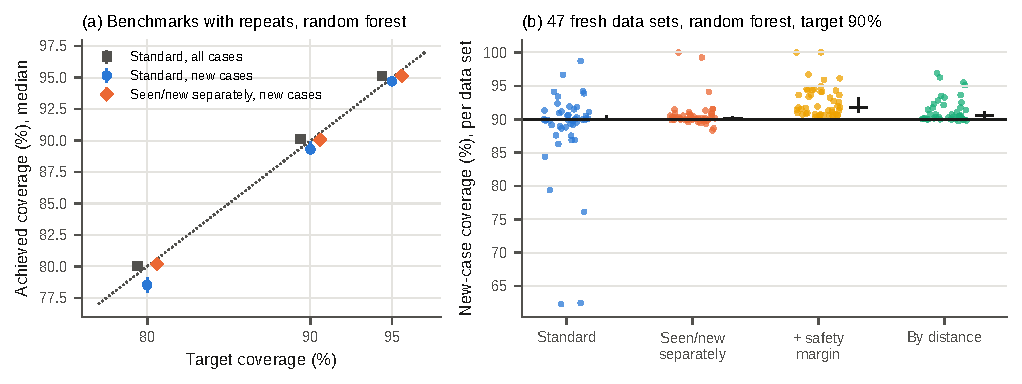
\includegraphics[width=\textwidth]{figures/fig_validity.pdf}
\caption{Target versus achieved coverage. (a) Benchmark data sets with repeats, random forest: standard calibration meets the target overall but not for new cases, while separate calibration meets it for new cases. Medians over data sets with 95\% bootstrap intervals. (b) The \NScpN{} fresh data sets at a 90\% target: new-case coverage per data set (dots) and medians with 95\% bootstrap intervals (black)}\label{fig:validity}
\end{figure}

\paragraph{H5--H7: the check on fresh data.}\label{sec:res-fresh} Figure~\ref{fig:screen} plots the predicted gap against the observed gap for all \NScpN{} fresh data sets.
\begin{itemize}
\item \emph{H5 (limit).} The predicted gap held as a limit. The random forest's gap stayed above $g^*-2$\,pp in \NPrRfAbove{}\% of wave-1 data sets (95\% CI \NPrRfAboveCi{}\%) and in \NWTwoRfAbove{}\% of wave-2 data sets (95\% CI \NWTwoRfAboveCi{}). The exception was \NWTwoViolNames{}.
\item \emph{H6 (ranking).} The predicted gap did \emph{not} rank the wave-1 data sets ($\rho$ = \NPrRfRho{}, Holm-adjusted $p$ = \NPrHolmPOne{}). Most of them have essentially no shortfall, so their ranks are decided by noise. It did rank the wave-2 data sets, which contain more real shortfalls ($\rho$ = \NWTwoRfRho{}, $p$ \NWTwoRfRhoP{}).
\item \emph{H7 (screening), the primary test of wave~2.} The combined flag caught all \NScTwoPos{} wave-2 data sets with a real shortfall (sensitivity \NScTwoSens{}, 95\% CI \NScTwoSensCi{}; Holm-adjusted $p$ = \NWTwoHolmWOne{}). Pooled over both waves, it caught \NScpHit{} of \NScpPos{} (95\% CI \NScpSensCi{}). Among the \NScpUnfl{} unflagged data sets, the worst gap for any learner was \NScpUnflWorst{}\,pp. The price is false alarms: specificity was \NScpSpec{}, but a false alarm only means applying a fix that costs almost nothing. The result depends little on where a ``real shortfall'' begins. With the flag rule unchanged, the check caught \NThrThreeHit{} shortfalls worse than $-3$\,pp and \NThrFiveHit{} worse than $-5$\,pp. With a looser threshold of $-1$\,pp it caught \NThrOneHit{}, missing three small shortfalls between $-1$ and $-2$\,pp (Supplementary Table~\ref{S-tab:threshold}).
\end{itemize}
The flagged shortfalls come from many domains. In wave~2 the random forest's gap was \NWTwodsSkinRf{}\,pp on skin segmentation, \NWTwodsDroidRf{}\,pp on Android malware permissions, \NWTwodsDiabRf{}\,pp on early diabetes risk and \NWTwodsVoteRf{}\,pp on voting records. LightGBM's gap on maternal health risk was \NWTwodsMatLgbm{}\,pp.

\begin{figure}[t]
\centering
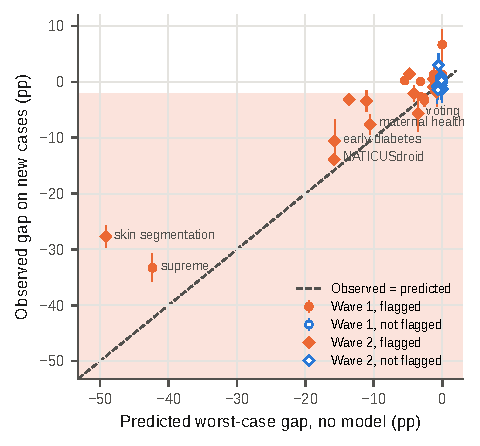
\includegraphics[width=0.62\textwidth]{figures/fig_screen.pdf}
\caption{On the \NScpN{} fresh data sets, every data set with a real shortfall (shaded, worse than $-2$\,pp) was flagged by the check before training. Observed gap: the worse of random forest and LightGBM, mean over 20 splits with a 95\% bootstrap interval. Filled markers: flagged; open markers: not flagged}\label{fig:screen}
\end{figure}

Label purity mattered in both directions. In black\_friday (\NPrBfPi{} of test rows seen), seattlecrime6 (\NPrScPi{}) and superconduct (\NPrCondPi{}), repeated rows almost never agree on the exact target. Exposure alone predicts gaps of \NPrBfGp{}, \NPrScGp{} and \NPrCondGp{}\,pp, while purity predicts none. The random forest's gaps were \NPrBfRfGap{}, \NPrScRfGap{} and \NPrCondRfGap{}\,pp. Over-coverage of new cases also has an explanation. On airlines, the predicted worst case was \NPrAirGs{}\,pp but the observed gap was \NPrAirRfGap{}\,pp. We had first attributed this to tied scores. The pre-specified tie-breaking test refuted that: with random tie-breaking, airlines' gap stayed at \NTbAirRand{}\,pp. Across the \NTbN{} highly exposed data sets, mean over-coverage fell only from \NTbOverScp{} to \NTbOverRand{}\,pp ($p$ = \NTbP{}). The data point instead to the mirror image of memorization. Seen airlines rows were covered only \NMirAirSeen{}\% of the time, because identical flight profiles carry conflicting delay labels. By Eq.~(\ref{eq:decomp}), new rows must then be over-covered (\NMirAirNew{}\%). Diabetes130US behaved the same way (seen \NMirDiaSeen{}\%, new \NMirDiaNew{}\%).

\paragraph{H8: the safety margin.} With separate calibration, \NPrFourRfMcp{}\% of wave-1 splits had new-case coverage below 87\% (random forest). With the safety margin this fell to \NPrFourRfPac{}\%; in wave~2 it fell from \NWTwoFixRfBad{}\% to \NWTwoPACMCPRfBad{}\%. Because most data sets had no unlucky splits at all, the planned wave-1 test was not significant after Holm correction ($p$ = \NPrHolmPFour{}). The margin enlarged sets by a factor of about \NPrSizePac{}.

\paragraph{H9: purity against exposure.} The advantage of purity over exposure alone for \emph{ranking} was not established on wave~1 (difference in $\rho$, 95\% CI \NPrRfDiffci{}). Its value lies in the screening decision, where it removes false alarms, as described above.

\paragraph{Is the variation just noise?} \emph{Post hoc.} Under exchangeability, the coverage of a split follows a known Beta--binomial law given the numbers of new calibration and test rows. We simulated it for every fresh split and compared the expected number of bad splits with the observed number (Supplementary Table~\ref{S-tab:noise}). For separate calibration with random forests, \NNoiseMCPRfObs{} bad splits were observed against \NNoiseMCPRfExp{} expected from pure noise (ratio \NNoiseMCPRfRatio{}, $p$ = \NNoiseMCPRfP{}). For standard calibration the ratio was \NNoiseSCPRfRatio{} ($p$ \NNoiseSCPRfP{}), so its shortfalls are real, not chance. LightGBM showed a small excess even with the fix (ratio \NNoiseMCPLgbmRatio{}, $p$ = \NNoiseMCPLgbmP{}), which we report but cannot explain with the data at hand.

\subsection{Qualitative analysis}\label{sec:res-qual}
\emph{Post hoc.} Table~\ref{tab:examples} shows mc1 test modules chosen by a fixed rule, never by hand. The rule takes the first seen module, the first four new modules in data-set order, the first new defective module and the first new module that the fix misses. The standard threshold is very strict (\NExQStd{}) because most calibration rows are memorized copies with score zero. The new-case threshold of the fix is \NExQNew{}. Module 44 shows the typical repair: an empty set becomes a correct set. The failure cases are as instructive. The first new \emph{defective} module receives an empty set from both methods.

\begin{table}[t]
\caption{mc1 test modules chosen by a fixed rule (random forest, first random split, 90\% target). LOC: lines of code; CC: cyclomatic complexity; $\hat p$: predicted defect probability; sets: N, no defect; D, defect; $\emptyset$, empty. \cmark/\xmark: set contains / misses the true label}\label{tab:examples}
\centering\scriptsize
\setlength{\tabcolsep}{3pt}
\begin{tabular}{@{}lrlrrlrll@{}}
\toprule
Rule & Row & Type & LOC & CC & True & $\hat p$ & Standard & Fixed\\
\midrule
\tabinput{tables/tab_examples.tex}
\botrule
\end{tabular}
\end{table}

This points to a limitation that matters for defect triage. Only \NMcOneDefShare{}\% of mc1 modules are defective, so a coverage promise over all new modules says little about the defective ones. Over 10 splits, new defective modules (\NCcFixDefN{} in total) were never covered, by standard calibration (\NCcStdDefCov{}\%) or by the fix (\NCcFixDefCov{}\%). Calibrating by seen/new \emph{and} by class, which is label-conditional Mondrian calibration \citep{lofstrom2015,vovk2022}, covered them \NCcClsDefCov{}\% of the time. The cost is that most new modules then receive both labels (mean set size \NCcClsOkSize{} against \NCcFixOkSize{}): the model admits that it cannot tell. For rare but important classes, the fix should therefore be combined with class-wise calibration, which the tool offers as an option (\texttt{classwise=True}).

\subsection{Ablation study}\label{sec:res-ablation}
Table~\ref{tab:ablation} removes one part of the routine at a time. For the check, exposure alone flags \NAblExpoFlag{} of the \NAblNds{} fresh data sets and purity alone \NAblPureFlag{}. The combined rule flags \NAblCombFlag{} and catches all \NAblNpos{} real shortfalls. Purity alone misses one, black\_friday with a linear model, because a linear model cannot memorize rows and the shortfall there has a different cause. For the fix, removing separate calibration brings the shortfall back (Fig.~\ref{fig:validity}). Robustness checks against the most obvious alternative explanations come next.
\begin{itemize}
\item \emph{Target level.} The pattern holds at 80\%, 90\% and 95\% (Fig.~\ref{fig:validity}a).
\item \emph{Tied scores.} Random tie-breaking does not remove the effect (above).
\item \emph{Hyperparameters.} Making random forests less flexible lowered seen-row coverage, but the change in the gap was too small to detect at benchmark exposures (trend $p$ = \NCapClassificationRfP{}). We therefore rely on the learner comparison of Fig.~\ref{fig:inject} for the role of flexibility.
\item \emph{Near-copies.} Copies with noise of 0.1\% of a standard deviation are invisible to exact matching: the planted-leak test flagged \NLeakJitterRecall{}\% of them, but \NLeakRecall{}\% of \NLeakPlanted{} exact copies with no false positives. The shortfall persisted: the random forest's gap on truly new cases was \NNdClaZeropZeroSCP{}\,pp with exact copies and \NNdClaZeropZeroZeroOneSCP{}, \NNdClaZeropZeroOneSCP{} and \NNdClaZeropOneSCP{}\,pp with noise of 0.1\%, 1\% and 10\% of a standard deviation (Fig.~\ref{fig:neardup}). Calibration by distance stayed at the target (\NNdClaZeropZeroDCP{}, \NNdClaZeropZeroZeroOneDCP{}, \NNdClaZeropZeroOneDCP{} and \NNdClaZeropOneDCP{}\,pp at the four noise levels) and matched an oracle that knows the true record identity.
\end{itemize}

\begin{table}[t]
\caption{Ablation of the check on the \NAblNds{} fresh data sets, against the \NAblNpos{} data sets with a real shortfall (random forest or LightGBM gap below $-2$\,pp). Flag rules: exposure only ($\bar\pi\ge0.10$ or exposure-based gap below $-2$\,pp); purity only ($g^*<-2$\,pp); combined (either)}\label{tab:ablation}
\centering\small
\begin{tabular}{@{}lrrrr@{}}
\toprule
Flag rule & Flagged & Shortfalls caught & Correct no-flags & False alarms\\
\midrule
Exposure only & \NAblExpoFlag{} & \NAblExpoSens{} & \NAblExpoSpec{} & \NAblExpoFa{}\\
Purity only ($g^*$) & \NAblPureFlag{} & \NAblPureSens{} & \NAblPureSpec{} & \NAblPureFa{}\\
Combined (used) & \NAblCombFlag{} & \NAblCombSens{} & \NAblCombSpec{} & \NAblCombFa{}\\
\botrule
\end{tabular}
\end{table}

\begin{figure}[t]
\centering
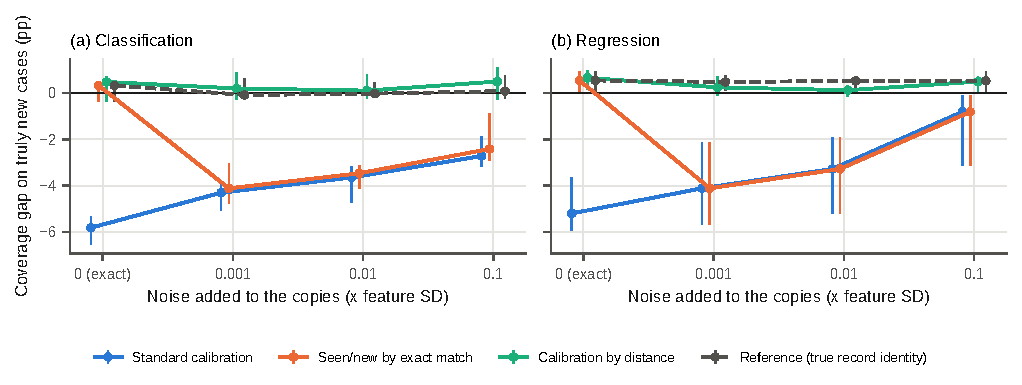
\includegraphics[width=\textwidth]{figures/fig_neardup.pdf}
\caption{Copies with a little noise defeat the exact-match check, and the shortfall persists; calibration by distance to the training rows stays on target and matches the oracle. Random forest, half of the rows copied, median over \NNdN{} data sets with 95\% bootstrap intervals}\label{fig:neardup}
\end{figure}

\subsection{Comparative analysis of remedies}\label{sec:res-remedies}
Figure~\ref{fig:remedies} and Table~\ref{tab:remedies} compare six options on the twelve application data sets, with the same splits and random forests (pre-specified, exploratory). What matters is which rows the calibration uses. Every remedy that calibrates on new rows brings new-case coverage to the target, and standard calibration does not. Removing repeats works about as well for new cases (\NRemDedupNewMed{}\% median), but it discards data: on mc1 the model is trained on \NRemMcOneTrainDedup{} instead of \NRemMcOneTrainFull{} modules. It also gives seen cases the sets calibrated for new ones, so they are over-covered (\NRemDedupSeenCov{}\%) with larger sets (\NRemDedupSeenSize{} against \NRemMCPSeenSize{} labels). A group split gives honest new-case coverage but says nothing about seen cases. On KDD Cup'99 it was infeasible in \NRemGscpKddFail{} splits, because a single group of identical connections exceeds the test part. Separate calibration keeps all data, works with any split and is valid for seen and new cases at once. In one small data set (mw1) fewer than nine seen calibration rows were available, so seen cases received the full set (Fig.~\ref{fig:remedies}b).

\begin{figure}[t]
\centering
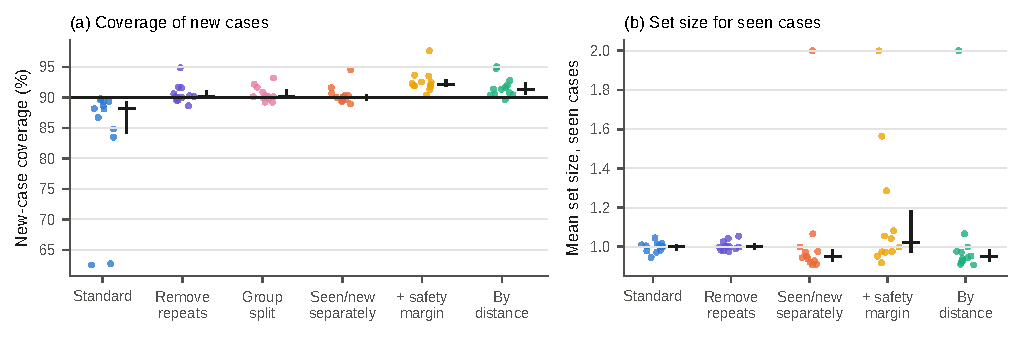
\includegraphics[width=\textwidth]{figures/fig_remedies.pdf}
\caption{Every remedy that calibrates on new rows reaches the target for new cases (a). Separate calibration does so without discarding data and gives seen cases smaller sets than removing repeats (b). Twelve application data sets, random forest, 10 splits; dots are data sets; black marks are medians with 95\% bootstrap intervals. The three points at 2.0 in (b) are mw1, where too few seen calibration rows exist}\label{fig:remedies}
\end{figure}

\begin{table}[t]
\caption{Remedies on the twelve application data sets (random forest, 90\% target, 10 random splits). New-case coverage: median and worst data set. Seen: coverage and mean set size for test rows with a training copy. Data used: median share of training rows kept}\label{tab:remedies}
\centering\footnotesize
\setlength{\tabcolsep}{3pt}
\begin{tabularx}{\textwidth}{@{}Xrrrrrr@{}}
\toprule
Method & \multicolumn{2}{c}{New-case coverage (\%)} & Empty sets & \multicolumn{2}{c}{Seen cases} & Data used\\
 & median & worst & new (\%) & cov. (\%) & size & (\%)\\
\midrule
\tabinput{tables/tab_remedies.tex}
\botrule
\end{tabularx}
\end{table}

\subsection{Computational complexity}\label{sec:res-cost}
The check hashes every row once and counts group sizes and label agreements. This is $O(N)$ hashing plus $O(N\log N)$ grouping, with memory linear in $N$. The fix adds one sort per group of calibration scores, $O(n_C\log n_C)$, the same order as standard split conformal prediction. Table~\ref{tab:cost} gives measured times on the stated machine. The check took at most \NCostCheckMax{}\,s and \NCostCheckMemMax{}\,MB on 30,000 rows. Calibration with the fix took the same time as standard calibration (at most \NCostCalExactMax{} against \NCostCalStdMax{}\,s), because model inference dominates.

\begin{table}[t]
\caption{Measured run time (median of five repetitions, seconds) and peak memory of the check, on \NHwNcpu{} logical CPUs (\NHwCpu{}). Model: fitting the random forest once. Calibration times include model inference on the calibration rows}\label{tab:cost}
\centering\footnotesize
\setlength{\tabcolsep}{3pt}
\begin{tabular}{@{}lrrrrrrrrr@{}}
\toprule
 & & & \multicolumn{2}{c}{Check} & Model & \multicolumn{3}{c}{Calibration} & Predict\\
Data & Rows & Feat. & s & MB & fit (s) & std & seen/new & distance & (s)\\
\midrule
\tabinput{tables/tab_cost.tex}
\botrule
\end{tabular}
\end{table}

\subsection{Case study: the tool on NASA mc1}\label{sec:case}
A practitioner who runs \texttt{covercheck mc1.csv --target defective} sees Fig.~\ref{fig:tool}. The check takes \NToolCheckS{}\,s and needs no model. It predicts a worst-case gap of \NToolGap{}\,pp, because \NToolPip{} of test modules will have a training copy with the same label, and it recommends the fix. The report then shows the problem directly: overall coverage of \NToolStdAll{}\%, but \NToolStdNew{}\% for new modules, \NToolStdEmpty{} of which receive an empty set. With the fix, new modules are covered \NToolFixNew{}\% of the time.

\emph{Real-world check of the tool.} \emph{Post hoc.} We ran the installed command-line tool, with its defaults, on \NTvN{} wave-2 data files downloaded fresh from the UCI repository. These were all wave-2 data sets with at most 30,000 rows, and the cached research pipeline was not used. The tool's exposure equalled the pipeline's to within $10^{\NTvExpDiffExp}$. Its verdicts agreed with the paper's rule on \NTvFlag{} of \NTvN{} files. Its new-case coverage agreed with the pipeline within two standard errors on \NTvFixTwose{} of \NTvN{} files (median difference \NTvMedFix{}\,pp), although preprocessing and seeds differ.

\begin{figure}[t]
\centering
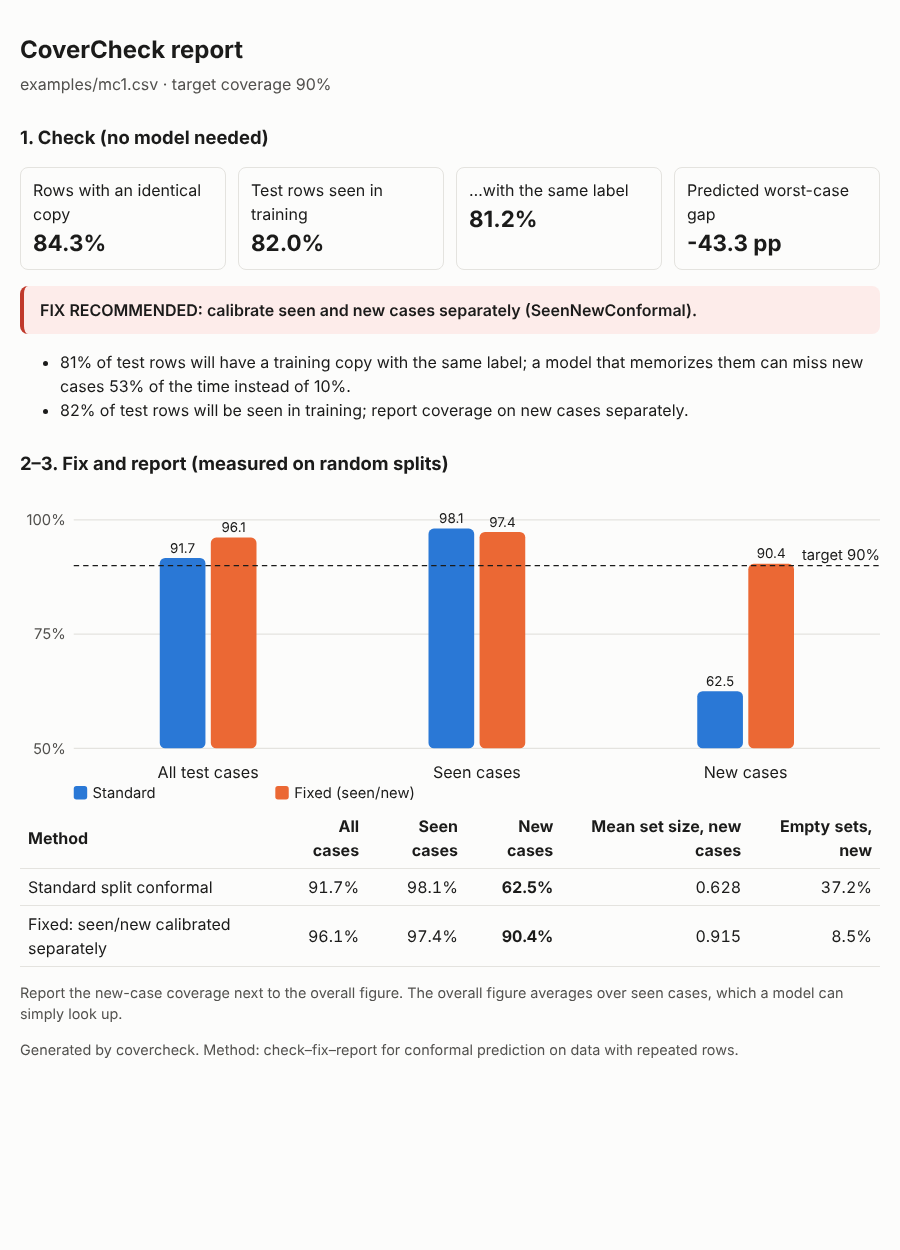
\includegraphics[width=0.78\textwidth]{figures/fig_tool.png}
\caption{The one-page report written by \emph{covercheck} for the NASA mc1 defect data: the check before training, its verdict, and measured coverage on all, seen and new cases with and without the fix. Random forest, 10 random splits}\label{fig:tool}
\end{figure}

\subsection{Discussion}\label{sec:discussion}
\paragraph{What a practitioner should do.} First, run the check before training. In our data, a predicted gap no worse than $-2$\,pp together with fewer than 10\% seen test rows meant that nothing needed to change; this rule was written down before the fresh data were analysed. Second, if the data set is flagged, calibrate seen and new cases separately. Add the safety margin when fewer than a few hundred new calibration rows exist, and use calibration by distance when near-copies are plausible. Third, report new-case coverage next to the overall figure. In defect triage, intrusion detection or clinical screening, the reported coverage decides how many cases go to manual review. An empty set for a new defect-prone module is a silent failure that no overall figure reveals.

\paragraph{Should one simply remove duplicates?} Not always. If the same input recurs in deployment, such as a frequent connection pattern, repeats are part of the population. Removing them discards data and gives over-cautious sets to recurring cases (Table~\ref{tab:remedies}). Separate calibration keeps the data and gives a valid promise for both kinds of case.

\paragraph{Limitations.}
\begin{enumerate}
\item \emph{Exact matching only.} The check sees only identical feature vectors. Near-copies need calibration by distance (Fig.~\ref{fig:neardup}), and choosing a coarser match, such as rounding, is a modelling decision.
\item \emph{The predicted gap is a limit and a screen, not a forecast.} It did not rank the wave-1 data sets (H6). It also fails in both directions when Assumption~\ref{as:equal} fails: a much larger shortfall when slightly differing repeats are still easy (solar\_flare in the benchmarks), and over-coverage when seen rows with conflicting labels are hard (airlines).
\item \emph{The typical benchmark is not affected} (H1), and varying flexibility within one learner was inconclusive. The problem is real but concentrated, which is why a check is useful.
\item \emph{Marginal over new cases, not per class.} A promise over all new cases does not protect a rare class (mc1 defects). Class-wise calibration is needed there, at the cost of larger sets.
\item \emph{Small calibration groups.} With few new calibration rows, coverage varies from split to split. The safety-margin effect was not significant after correction (H8), and LightGBM showed a small excess of bad splits that we cannot explain.
\item \emph{No time order.} All splits are random. The NASA, intrusion and phishing data carry no time stamps, so we could not test a deployment in which new releases arrive over time.
\item \emph{Few regression data sets in wave~2.} The second fresh collection is almost all classification (\NWTwoNCls{} of \NWTwoN{}). Regression evidence comes from the benchmarks, wave~1 and the copy experiments.
\item \emph{Same population.} Coverage on held-out new rows equals coverage on future records only if they come from the same population. Distribution shift needs other tools \citep{tibshirani2019,barber2023}.
\item \emph{Study conduct.} Several analyses were added after results were seen and are labelled post hoc, and the plans were amended during the study (D1--D17). The work was done with substantial AI assistance (Sect.~\ref{sec:framework}).
\end{enumerate}
